\documentclass[
  article,
  12pt,
  oneside,
  a4paper,
  english,
  brazil,
  chapter=TITLE,
  section=TITLE,
  subsection=TITLE
]{abntex2}

\usepackage[T1]{fontenc}
\usepackage[utf8]{inputenc}
\usepackage{newtxtext,newtxmath}
\usepackage{indentfirst}
\usepackage{graphicx}
\usepackage{microtype}
\usepackage{placeins}
\usepackage{listingsutf8}

\lstset{
  inputencoding=utf8/latin1,
  language=Python,
  basicstyle=\ttfamily\footnotesize,
  breaklines=true,
  columns=fullflexible,
  keepspaces=true,
  showstringspaces=false,
  tabsize=2,
  frame=single,
  numbers=left,
  numberstyle=\tiny,
  numbersep=8pt,
  xleftmargin=2em,
  framexleftmargin=1.6em,
  aboveskip=8pt,
  belowskip=8pt
}

\makeatletter
\g@addto@macro{\UrlBreaks}{\do\_}
\makeatother

\titulo{Classificação do impacto das redes sociais com Naive Bayes e árvore de decisão}
\autor{Ian de Araújo \and Jardson Alan}
\local{Rio Grande do Norte}
\data{2026}
\instituicao{%
  Instituto Federal de Educação, Ciência e Tecnologia\\
  do Rio Grande do Norte%
}
\preambulo{%
  Artigo apresentado à disciplina de Análise de Dados do Instituto Federal
  de Educação, Ciência e Tecnologia do Rio Grande do Norte, com o registro
  da etapa de classificação do projeto.%
}

\hypersetup{
  hidelinks,
  pdftitle={Classificação do impacto das redes sociais com Naive Bayes e árvore de decisão},
  pdfauthor={Ian de Araújo; Jardson Alan}
}

\renewcommand{\imprimircapa}{%
  \begin{capa}%
    \SingleSpacing
    \begin{center}
      \imprimirinstituicao\par
      \vspace*{\fill}
      \imprimirautor\par
      \vspace*{\fill}
      {\bfseries\imprimirtitulo\par}
      \vspace*{\fill}
      \imprimirlocal\par
      \imprimirdata\par
    \end{center}
    \vspace*{1cm}
  \end{capa}%
}

\renewcommand{\folhaderostocontent}{%
  \SingleSpacing
  \begin{center}
    \imprimirautor\par
  \end{center}
  \vspace{3.2cm}
  \begin{center}
    {\bfseries\imprimirtitulo\par}
  \end{center}
  \vspace{2.2cm}
  \hfill
  \begin{minipage}[t]{.46\textwidth}
    \imprimirpreambulo
  \end{minipage}
  \vspace{3.2cm}
  \begin{center}
    \imprimirlocal\par
    \imprimirdata\par
  \end{center}
}

\AtBeginDocument{%
  \setlength{\absleftindent}{0pt}%
  \setlength{\absrightindent}{0pt}%
  \setlength{\absparindent}{0pt}%
  \setlength{\emergencystretch}{2.5em}%
}

\graphicspath{{../figures/}}

\begin{document}

\pretextual
\imprimircapa
\imprimirfolhaderosto

\textual

\begin{center}
  \bfseries\imprimirtitulo
\end{center}

\vspace{0.75\baselineskip}
\noindent Ian de Araújo\footnotemark{} e Jardson Alan\footnotemark[\value{footnote}]
\footnotetext{Estudantes da disciplina de Análise de Dados do Instituto Federal de Educação, Ciência e Tecnologia do Rio Grande do Norte.}

\begin{resumo}
Esta etapa classifica o impacto das redes sociais em 4.500 estudantes. A classe é \texttt{Overall\_Impact}, com os rótulos \texttt{Beneficial}, \texttt{Neutral} e \texttt{Negative}. As entradas são sete medidas numéricas, as mesmas do agrupamento, e o índice de saúde mental fica de fora. O Naive Bayes gaussiano é avaliado por validação cruzada de cinco partes, com acurácia média de 0,9238. A árvore de decisão passa por \texttt{GridSearchCV} no recorte de treino. Os hiperparâmetros escolhidos são critério de Gini, profundidade máxima 7, mínimo de 10 amostras para dividir um nó e mínimo de 4 amostras na folha. Com esses parâmetros, a validação cruzada da árvore chega a 0,9480. Os dois resultados usam \texttt{cross\_val\_score}.

\vspace{\onelineskip}
\noindent
\textbf{Palavras-chave}: Classificação. Naive Bayes. Árvore de decisão. Validação cruzada. Redes sociais.
\end{resumo}

\section{Etapa de classificação}

O objetivo é prever a classe já existente em \texttt{Overall\_Impact}. Há 3.681 registros \texttt{Beneficial}, 654 \texttt{Neutral} e 165 \texttt{Negative}, como na Figura~\ref{fig:classes}. O arquivo é \texttt{data/raw/}\allowbreak\texttt{dataset.csv}, com 4.500 estudantes (YADAV, 2026).

\begin{figure}[htb]
  \centering
  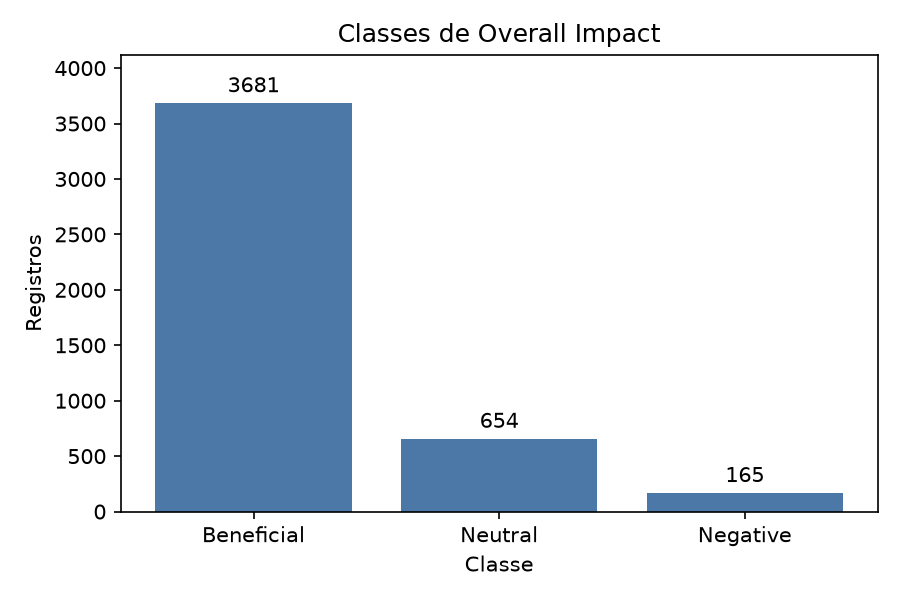
\includegraphics[width=0.85\textwidth]{class_counts.png}
  \caption{Contagem das classes de \texttt{Overall\_Impact}}
  \label{fig:classes}
  \fonte{Elaborado pelos autores (2026), pela execução dos classificadores.}
\end{figure}

As entradas vêm de \texttt{prepare\_data}, em \texttt{src/clustering/}\allowbreak\texttt{grouping.py}: idade, horas diárias, horas extras de fim de semana, duração e qualidade do sono, estresse percebido e GPA. Os vazios de estresse e de GPA recebem a média truncada por idade. \texttt{Student\_ID} e \texttt{Mental\_Health\_Index} não entram. A classe também não entra como variável.

Os dois classificadores usam o mesmo recorte, com 33\% dos registros para teste e semente 125. A comparação exigida pela etapa, porém, é a validação cruzada de cinco partes, com acurácia, aplicada aos dois modelos por \texttt{cross\_val\_score}.

\section{Naive Bayes}

O modelo é o \texttt{GaussianNB}, adequado às colunas numéricas. Não há busca de hiperparâmetros. A Tabela~\ref{tab:cv} mostra os cinco resultados e a média de 0,9238, com desvio-padrão de 0,0090. No recorte de teste, a acurácia foi 0,9178.

\begin{table}[htb]
  \centering
  \caption{Acurácia na validação cruzada de cinco partes}
  \label{tab:cv}
  \small
  \begin{tabular}{lrrrrr}
    \toprule
    Modelo & Parte 1 & Parte 2 & Parte 3 & Parte 4 & Parte 5 \\
    \midrule
    Naive Bayes & 0,9278 & 0,9289 & 0,9233 & 0,9067 & 0,9322 \\
    Árvore de decisão & 0,9544 & 0,9444 & 0,9556 & 0,9356 & 0,9500 \\
    \bottomrule
  \end{tabular}
  \fonte{Elaborado pelos autores (2026), pela execução dos classificadores.}
\end{table}

A Figura~\ref{fig:cv} mostra as mesmas cinco partes. O eixo começa em 0,85 para a diferença entre os modelos aparecer. Em todas as partes a árvore fica acima do Naive Bayes.

\begin{figure}[htb]
  \centering
  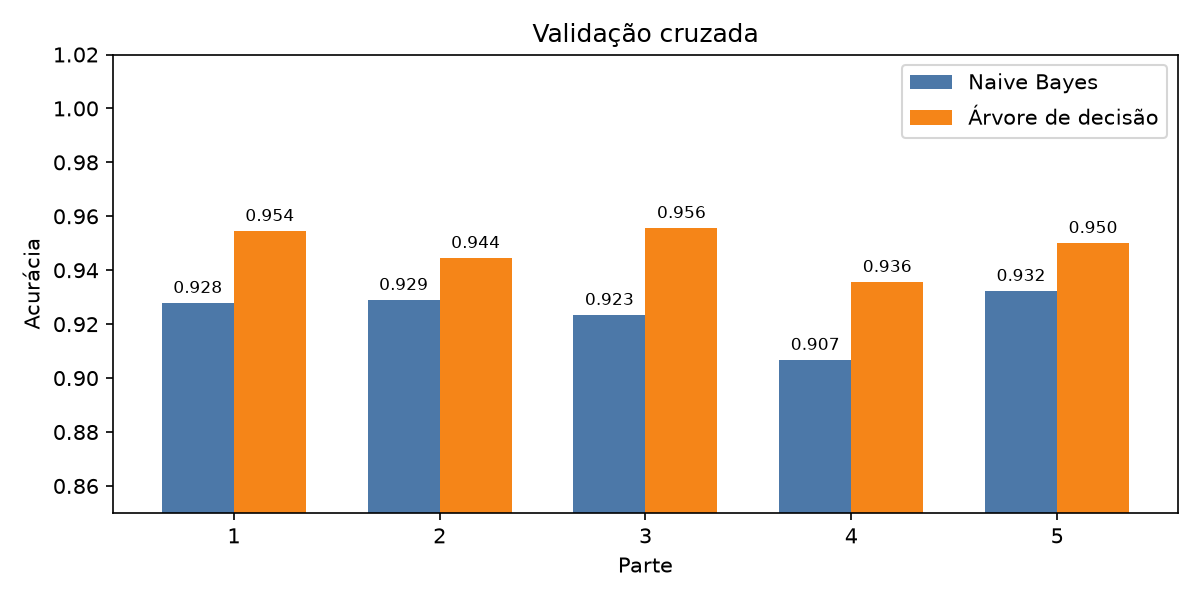
\includegraphics[width=\textwidth]{cross_validation.png}
  \caption{Acurácia nas cinco partes da validação cruzada}
  \label{fig:cv}
  \fonte{Elaborado pelos autores (2026), pela execução dos classificadores.}
\end{figure}

A Tabela~\ref{tab:nb} é a matriz do recorte de teste. Os 52 registros \texttt{Negative} desse recorte foram quase todos reconhecidos: 49 acertos. Dos 229 \texttt{Neutral}, 194 foram previstos nessa classe. A maior troca ocorre entre \texttt{Beneficial} e \texttt{Neutral}.

\begin{table}[htb]
  \centering
  \caption{Matriz do Naive Bayes no recorte de teste}
  \label{tab:nb}
  \begin{tabular}{lrrr}
    \toprule
    Real & Beneficial & Negative & Neutral \\
    \midrule
    Beneficial & 1120 & 0 & 84 \\
    Negative & 0 & 49 & 3 \\
    Neutral & 14 & 21 & 194 \\
    \bottomrule
  \end{tabular}
  \fonte{Elaborado pelos autores (2026), pela execução dos classificadores.}
\end{table}

\section{Árvore de decisão}

O \texttt{GridSearchCV} ajusta a árvore só no recorte de treino. A grade combina critério \texttt{gini} ou \texttt{entropy}, profundidade máxima 3, 5, 7, 10 ou sem limite, mínimo de 2, 5 ou 10 amostras para dividir um nó e mínimo de 1, 2 ou 4 amostras na folha. São cinco partes internas e o critério da busca é a acurácia. A semente é 125.

O conjunto escolhido foi critério de Gini, profundidade máxima 7, mínimo de 10 amostras para dividir e mínimo de 4 amostras na folha. Uma árvore nova, com esses hiperparâmetros, foi avaliada por \texttt{cross\_val\_score} no conjunto inteiro. A média foi 0,9480 e o desvio-padrão 0,0074, como na Tabela~\ref{tab:cv}. No recorte de teste, a acurácia foi 0,9434.

\begin{table}[htb]
  \centering
  \caption{Matriz da árvore de decisão no recorte de teste}
  \label{tab:tree}
  \begin{tabular}{lrrr}
    \toprule
    Real & Beneficial & Negative & Neutral \\
    \midrule
    Beneficial & 1186 & 0 & 18 \\
    Negative & 0 & 44 & 8 \\
    Neutral & 51 & 7 & 171 \\
    \bottomrule
  \end{tabular}
  \fonte{Elaborado pelos autores (2026), pela execução dos classificadores.}
\end{table}

Na Tabela~\ref{tab:tree} e na Figura~\ref{fig:matrizes}, a árvore acerta 1.186 dos 1.204 \texttt{Beneficial} do teste e 44 dos 52 \texttt{Negative}. O \texttt{Neutral} é a classe mais confundida: 51 desses registros foram previstos como \texttt{Beneficial}.

\begin{figure}[htb]
  \centering
  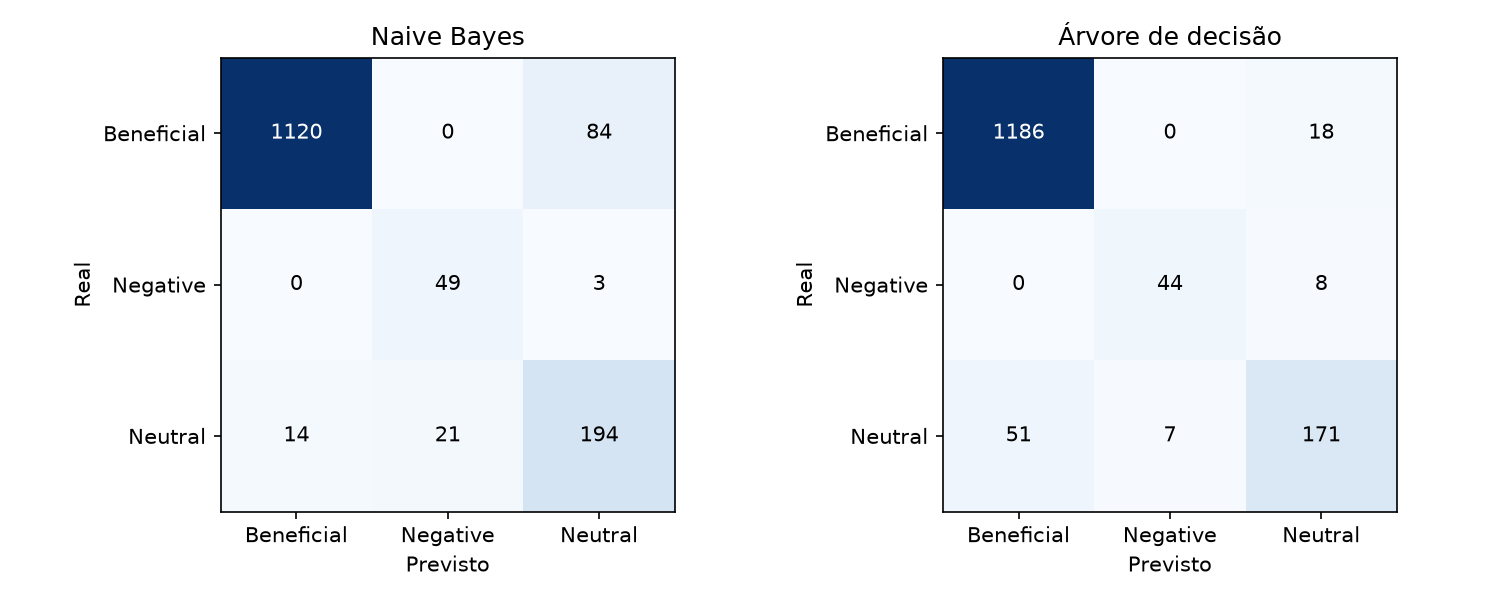
\includegraphics[width=\textwidth]{confusion_matrices.png}
  \caption{Matrizes de confusão no recorte de teste}
  \label{fig:matrizes}
  \fonte{Elaborado pelos autores (2026), pela execução dos classificadores.}
\end{figure}

\section{Comparativo}

Pela validação cruzada, a árvore fica acima do Naive Bayes em todas as cinco partes. A média passa de 0,9238 para 0,9480. O desvio-padrão também é menor, 0,0074 contra 0,0090. A classe \texttt{Beneficial} é a maioria do arquivo, então a acurácia dos dois já parte de um patamar alto. A diferença aparece sobretudo nela: a árvore troca menos \texttt{Beneficial} com \texttt{Neutral}. O Naive Bayes, no recorte de teste, recupera um pouco mais os \texttt{Negative} (49 contra 44).

\FloatBarrier

\section{Código utilizado}

As listagens são os arquivos desta etapa, como estão no repositório. \texttt{main.py} chama os dois classificadores e a função que grava as figuras. \texttt{naive\_bayes.py} avalia o \texttt{GaussianNB} com \texttt{cross\_val\_score}. \texttt{tree\_decision.py} escolhe os hiperparâmetros com \texttt{GridSearchCV} e avalia a árvore escolhida também com \texttt{cross\_val\_score}. \texttt{charts.py} grava os três gráficos em \texttt{reports/figures/}.

\subsection{Chamada no fluxo}

Arquivo \texttt{main.py}.

\lstinputlisting{../../../main.py}

\subsection{Naive Bayes}

Arquivo \texttt{src/classifiers/}\allowbreak\texttt{naive\_bayes.py}.

\lstinputlisting{../../../src/classifiers/naive_bayes.py}

\subsection{Árvore de decisão}

Arquivo \texttt{src/classifiers/}\allowbreak\texttt{tree\_decision.py}.

\lstinputlisting{../../../src/classifiers/tree_decision.py}

\subsection{Gráficos}

Arquivo \texttt{src/visualization/}\allowbreak\texttt{charts.py}.

\lstinputlisting{../../../src/visualization/charts.py}

\postextual

\begin{thebibliography}{9}
\bibitem{yadav2026}
YADAV, Harish. \textbf{Impact of Social Media on Life}. 2026. Conjunto de dados. Disponível em: \url{https://www.kaggle.com/datasets/harishyadav0506/impact-of-social-media-on-life}. Acesso em: 9 nov. 2026.
\end{thebibliography}

\end{document}
